
\section*{Problema P6.25}

\renewcommand*\thesection{6.25}
\numberwithin{equation}{section}

\begin{center}
    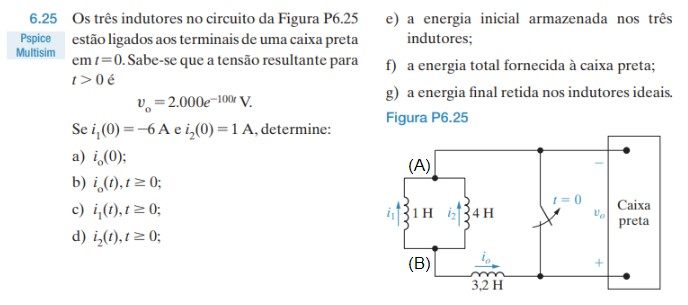
\includegraphics[scale=1.0]{P6.25.jpg}
\end{center}

\subsection*{(a)}

Aplicando análise nodal no nó essencial (B), temos

\[ i_0(t) + i_1(t) + i_2(t) = 0 \logo i_0(t) = - i_1(t) - i_2(t)  \]

Substituindo no instante $t=0$,

\[ i_0(0) = -(-6) - 1   \]

\[ \boxed{i_0(0) = 5 \un{A}}  \]

\subsection*{(b)}

Reduzindo os três indutores da figura via redução série-paralelo, temos um indutor equivalente $L_{eq}$ dado por 

\[ L_{eq} = (1\un{H} \;//\; 4\un{H}) + 3.2\un{H}  \]

\[ L_{eq} = 4.0\un{H}  \]

Assim, usando a expressão da corrente no indutor

\begin{equation}\label{eq:6.25.1}
    i(t) = i_0 + \frac{1}{L} \int_{t_i}^{t_f} v_L(t) \,dt
\end{equation}

Note que no sentido em que $i_o(t)$ está definida na figura, temos, via análise de malhas,

\[+v_o(t) + v_{L_{eq}}(t) = 0  \logo  v_{L_{eq}}(t) = - v_o(t) \]

Assim, temos que \eqref{eq:6.25.1} deve ter o sinal ajustado para atender a convenção passiva definida acima, ficando

\begin{equation}\label{eq:6.25.2}
    i(t) = i_0 - \frac{1}{L} \int_{t_i}^{t_f} v_0(t) \,dt
\end{equation}

Substituindo os valores do enunciado e resultado do item (a) em \eqref{eq:6.25.2}, temos

\[ i(t) = 5 - \frac{1}{4}\int_{0}^{t} 2000e^{-100t} \,dt  \]

\[ i(t) = 5 - 2000\frac{1}{4}\frac{1}{-100}\left[e^{-100t} - e^{0}\right]  \]

\[ i(t) = 5 + 5\left[e^{-100t} - 1\right]  \]

\[ \boxed{i(t) = 5e^{-100t} \quad ,  \quad t > 0}  \]

\subsection*{(c)}

Retornando ao circuito original, temos que a queda de tensão no indutor de 


